\documentclass[a4paper, 12pt, openany]{book}
\usepackage[utf8]{vietnam}
\usepackage[vietnamese]{babel}
\usepackage{hyperref}
\usepackage{lipsum}
\usepackage[headings]{fullpage}
\usepackage{multicol}
\usepackage{fancyhdr}
\usepackage{indentfirst}
\usepackage{mathptmx}
\usepackage[style=ieee]{biblatex}
\usepackage[table]{xcolor}
\usepackage{pgfplots}
\usepackage{subcaption}
\usepackage{tikz}
\usepackage{floatrow}
\usepackage{acro}
\usepackage{amssymb}
\usepackage{amsmath}
\usepackage{afterpage}



\colorlet{punct}{red!60!black}
\definecolor{background}{HTML}{EEEEEE}
\definecolor{delim}{RGB}{20,105,176}
\colorlet{numb}{magenta!60!black}


\DeclareAcronym{rag}{
  short=RAG,
  long=Retrieval-Augmented Generation,
}

\DeclareAcronym{nlp}{
  short=NLP,
  long=Natural Language Processing,
}

\DeclareAcronym{cnn}{
  short=CNN,
  long=Convolutional Neural Network,
}

\DeclareAcronym{rnn}{
  short=RNN,
  long=Recurrent Neural Network,
}

\DeclareAcronym{gru}{
  short=GRU,
  long=Gated Recurrent Unit,
}

\DeclareAcronym{seq2seq}{
  short=Seq2Seq,
  long= Sequence to Sequence
}

\DeclareAcronym{mlm}{
  short=MLM,
  long=Masked Language Modeling,
}

\DeclareAcronym{nsp}{
  short=NSP,
  long=Next Sequence Prediction,
}

\DeclareAcronym{bert}{
  short=BERT,
  long=Bidirectional Encoder Representations from Transformers,
}

\DeclareAcronym{llm}{
  short=LLM,
  long=Large Language Model
}

% \newacronym{rag}{RAG}{Retrieval-Augmented Generation}
% \newacronym{nlp}{NLP}{Natural Language Processing}
% \newacronym{bert}{BERT}{Bidirectional Encoder Representations from Transformers}


\addbibresource{references.bib}

\pagestyle{fancy}
\fancyhead{}
\fancyfoot{}

\renewcommand{\headrulewidth}{0pt}


\fancyhead[L]{\leftmark}
\fancyhead[R]{\rightmark}
\fancyfoot[LO, RE]{\thepage}

\title{Luận văn tốt nghiệp}
\author{Trần Gia Huy}

\begin{document}

\fontfamily{ptm} % Set font family

\maketitle

% =======================================================================

\begin{center}
    \bf BỘ GIÁO DỤC VÀ ĐÀO TẠO

    TRƯỜNG ĐẠI HỌC CẦN THƠ

    TRƯỜNG CÔNG NGHỆ THÔNG TIN VÀ TRUYỀN THÔNG

    \vspace{2cm}

    TRẦN GIA HUY

    MÃ SỐ SINH VIÊN: B2016968

    \vspace{2cm}

    {\large
        HỖ TRỢ TƯ VẤN THỦ TỤC HÀNH CHÍNH TẠI CẦN THƠ BẰNG PHƯƠNG PHÁP RAG

        \vspace{1cm}
        ADVISE ADMINISTRATIVE PROCEDURES IN CAN THO CITY USING RAG METHOD
    }

    \vspace{2cm}

    LUẬN VĂN TỐT NGHIỆP

    NGÀNH: KHOA HỌC MÁY TÍNH

    MÃ SỐ: 748 101

    \vspace{2cm}

    GIẢNG VIÊN HƯỚNG DẪN

    PGS. TS. GVCC. PHẠM NGUYÊN KHANG

    \vspace{4cm}

    NĂM 2024
\end{center}
\newpage

% =======================================================================

\begin{center}
    TRƯỜNG CÔNG NGHỆ THÔNG TIN VÀ TRUYỀN THÔNG

    \textbf{KHOA KHOA HỌC MÁY TÍNH}

    \vspace{1.5cm}

    \textbf{\large XÁC NHẬN CHỈNH SỬA LUẬN VĂN \\ THEO Ý KIẾN CỦA HỘI ĐỒNG}
\end{center}

{
\noindent
Tên luận văn: Hỗ trợ tư vấn thủ tục hành chính tại Cần Thơ bằng phương pháp RAG và kiến trúc Microservices. (Advise administrative procedures in Can Tho using RAG method and Microservices architecture.).

\noindent
Họ tên sinh viên: Trần Gia Huy -- Mã số sinh viên: B2016968.

\noindent
Mã lớp: DI20Z6A1.

\noindent
Đã báo cáo tại hội đồng: Khoa học máy tính.

\noindent
Ngày báo cáo: --/--/----.

\noindent
Hội đồng báo cáo gồm: % # TODO: Hội đồng báo cáo gồm
\begin{enumerate}
    \item -------- -- Chủ tịch hội đồng.
    \item -------- -- Thành viên.
    \item -------- -- Thư ký.
\end{enumerate}

\noindent
Luận văn này đã được chỉnh sửa theo góp ý của Hội đồng.


\begin{multicols}{2}
    \begin{minipage}{\linewidth}
    \end{minipage}

    \begin{minipage}{\linewidth}
        \centering
        Cần Thơ, ngày -- tháng -- năm 2024 % # TODO: Ngày tháng năm

        \textbf{Giảng viên hướng dẫn}

        (Ký, ghi rõ họ tên) \\

        \vspace{2.5cm}

        Phạm Nguyên Khang
    \end{minipage}
\end{multicols}
}
\newpage

% =======================================================================


\chapter*{Lời cảm ơn}
\addcontentsline{toc}{chapter}{Lời cảm ơn}
Tôi xin gửi lời cảm ơn tới PGS. TS. GVCC. Phạm Nguyên Khang người đã tận tình giúp đỡ tôi trong quá trình học tập, nghiên cứu và hoàn thành luận văn này.

Tôi xin bày tỏ lòng biết ơn đến các Thầy Cô trong Khoa Khoa học máy tính, các Thầy Cô giảng dạy tại Trường Công nghệ thông tin và Truyền thông, Trường Đại học Cần Thơ đã giúp đỡ tôi trong suốt quá trình học tập và nghiên cứu tại Trường.

Sau cùng tôi xin gửi lời cảm ơn đến gia đình và bạn bè đã luôn ủng hộ tôi, động viên cũng như giúp đỡ tôi trong suốt thời gian qua.

Trong quá trình nghiên cứu và thực hiện đề tài luận văn sẽ không tránh khỏi nhiều sai sót và hạn chế, kính mong nhận được sự chỉ dẫn và đóng góp của quý Thầy Cô để bài luận văn của tôi được hoàn thiện hơn.

Tôi xin chân thành cảm ơn!

\begin{multicols}{2}
    \begin{minipage}{\linewidth}
    \end{minipage}

    \begin{minipage}{\linewidth}
        \begin{center}
            Cần Thơ, ngày -- tháng -- năm 2024 % # TODO: Ngày tháng năm

            \textbf{Tác giả}

            \vspace{2.5cm}

            Trần Gia Huy
        \end{center}
    \end{minipage}
\end{multicols}

% =======================================================================

\chapter*{Tóm tắt}
\addcontentsline{toc}{chapter}{Tóm tắt}
% # TODO: Tóm tắt

\chapter*{Abstract}
\addcontentsline{toc}{chapter}{Abstract}
% # TODO: Abstract

\chapter*{Lời cam đoan}
\addcontentsline{toc}{chapter}{Lời cam đoan}
Chúng tôi xin cam đoan Luận văn tốt nghiệp "Hỗ trợ tư vấn thủ tục hành chính tại Cần Thơ bằng phương pháp RAG và kiến trúc Microservices" \space là công trình nghiên cứu của riêng chúng tôi.
Ngoài các trích dẫn, tài liệu tham khảo đã được ghi nguồn đầy đủ.
Các số liệu, kết quả nêu trong luận văn là trung thực và chưa từng được công bố trong các công trình khác.
Nếu không đúng như đã nêu trên, chúng tôi xin hoàn toàn chịu trách nhiệm về đề tài của mình.

\begin{multicols}{2}
    \begin{minipage}{\linewidth}
    \end{minipage}

    \begin{minipage}{\linewidth}
        \centering
        Cần Thơ, ngày -- tháng -- năm 2024 % # TODO: Ngày tháng năm

        \textbf{Người cam đoan}

        (Ký, ghi rõ họ tên) \\

        \vspace{2.5cm}

        Trần Gia Huy
    \end{minipage}
\end{multicols}

\tableofcontents
\listoffigures
\listoftables


\printacronyms[name={Danh mục từ viết tắt}]

\renewcommand{\headrulewidth}{1pt} % Reset headrulewidth

\chapter{Giới thiệu}

\section{Lý do chọn đề tài}
% # TODO: Lý do chọn đề tài

\section{Mục tiêu nghiên cứu}
% # TODO: Mục tiêu đề tài

\section{Các nghiên cứu liên quan}
% # TODO: Các nghiên cứu liên quan

\section{Đối tượng và phạm vi nghiên cứu}
% # TODO: Đối tượng và phạm vi nghiên cứu

\section{Phương pháp nghiên cứu}
% # TODO: Phương pháp nghiên cứu

\section{Cấu trúc luận văn}
% # TODO: Cấu trúc luận văn
Nội dung luận văn bao gồm 3 chương:


\begin{itemize}
    \item \textbf{Chương 1 -- Giới thiệu:} Giới thiệu tổng quan về đề tài, mục tiêu, các phương pháp nghiên cứu, đối tượng và phạm vi nghiên cứu của đề tài.
    Chương này cũng sẽ giới thiệu sơ lược về khả năng ứng dụng của xử lý ngôn ngữ tự nhiên vào bài toán thực tế - cụ thể là hệ thống hỏi đáp về thủ
    tục hành chính ở địa bàn Cần Thơ.
    \item \textbf{Chương 2 -- Nội dung:} gồm 3 phần:
          \begin{itemize}
              \item \textbf{Phần 1 -- Cơ sở lý thuyết}: Phần này sẽ đi sâu vào các cơ sở lý thuyết của các giải pháp đã được áp dụng vào hệ thống hỏi đáp thủ tục hành chính.
              Các khái niệm và lý thuyết sẽ được đề cập đến bao gồm các phương pháp nhúng từ, mô hình Seq2Seq, kiến trúc Transformer, mô hình BERT, 
              độ tương đồng ngữ nghĩa Cosine, mạng sinh đôi (Siamese network), mô hình SBERT, RAG và các phương pháp có liên quan, cách đánh giá kết quả truy vấn thông tin.
              \item \textbf{Phần 2 -- Phương pháp thực hiện}: Phần này sẽ miêu tả cách thực hiện hệ thống hỏi đáp về thủ tục hành chính dựa trên RAG, cách xây dựng giải pháp và huấn luyện mô hình.
              \item \textbf{Phần 3 -- Kết quả thực nghiệm}: Phần này sẽ mô tả cách đánh giá các giải pháp, tiến hành thực nghiệm trên mô hình, kết quả đạt được sau khi
              đánh giá mô hình. 
          \end{itemize}
    \item \textbf{Chương 3 -- Kết luận:}: Phần này sẽ tổng kết kết quả đạt được của đề tài, nhận định về kết quả và một số hướng phát triển.
\end{itemize}

\chapter{Nội dung}

\section{Cơ sở lý thuyết}
\subsection{Xử lý ngôn ngữ tự nhiên}
% # TODO: Xử lý ngôn ngữ tự nhiên

\subsection{Phương pháp nhúng từ và văn bản}
% # TODO: Phương pháp nhúng từ và văn bản

\subsection{Mô hình Seq2Seq và cơ chế attention}
% # TODO: Mô hình Seq2Seq và cơ chế attention

\subsection{Mô hình Transformer}
\subsection{Kiến trúc Transformer}
\subsubsection{Tổng Quan}

Transformer\cite{Wolf2019HuggingFacesTS} là một mô hình học sâu được giới thiệu bởi Vaswani và các cộng sự [9]
vào năm 2017, đây là mô hình đã đạt được kết quả nổi bật trong nhiều nhiệm vụ xử lý
ngôn ngữ tự nhiên (NLP). Transformer được xây dựng dựa trên cơ chế Attention
(Attention mechanism, tạm dịch: cơ chế tập trung), cho phép mô hình có khả năng “tập
trung” vào các phần khác nhau của đầu vào (Input) trong quá trình học.

Mô hình Transformer sử dụng kiến thức đa đầu vào (Multi-Head Input) và đa đầu
ra (Multi-Head Output) để xử lý đầu vào và đầu ra theo cách đồng thời, tức là không cần
xử lý tuần tự từng phần như các mô hình trước đây. Điều này giúp giải quyết vấn đề độ
dài phụ thuộc trong ngôn ngữ (Long-range Dependency) và giúp mô hình có khả năng
hiểu ngữ cảnh (Contextual Understanding) của dữ liệu đầu vào (Input).

Mô hình Transformer đã được ứng dụng rộng rãi trong nhiều tác vụ xử lý ngôn ngữ
tự nhiên, bao gồm dịch máy, phân loại văn bản, dự đoán từ, tóm tắt văn bản, hỏi đáp, và
nhiều tác vụ ngôn ngữ tự nhiên khác. BERT\cite{devlin2019bert} (Bidirectional Encoder Representations from
Transformers), GPT\cite{brown2020language} (Generative Pre-trained Transformer), và T5\cite{raffel2023exploring} (Text-to-Text Transfer
Transformer) là những mô hình NLP nổi tiếng được xây dựng trên kiến trúc của mô hình
Transformer.

\begin{minipage}{\linewidth}
    \captionsetup{type=figure}
    \centering
    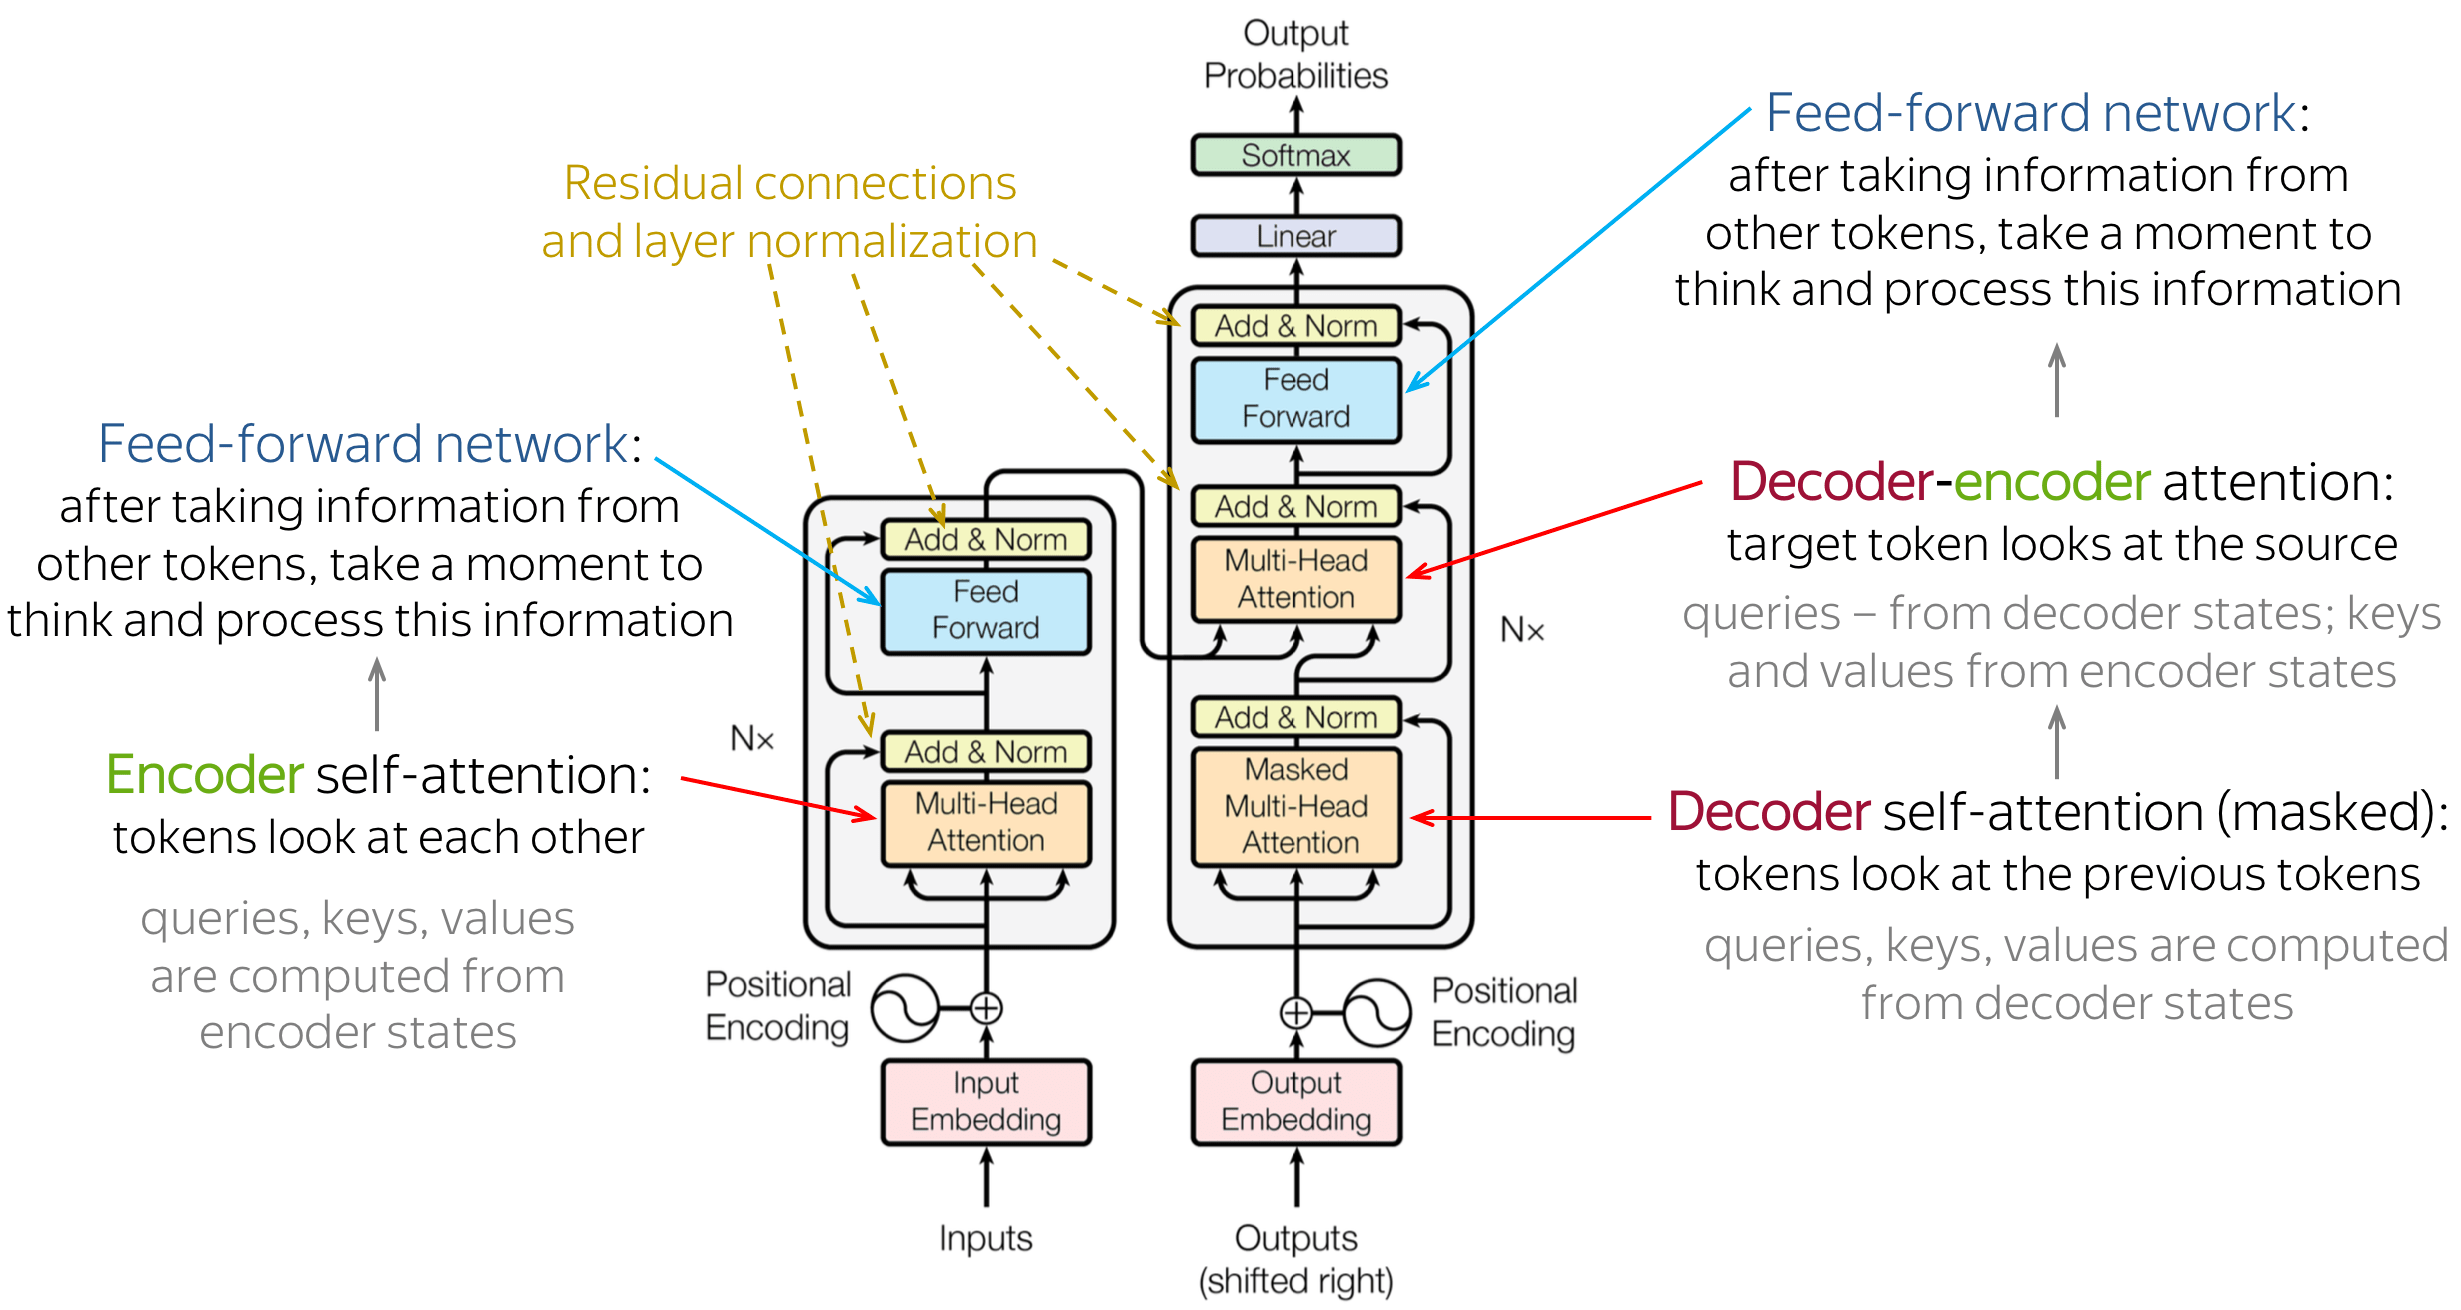
\includegraphics[width=\linewidth]{./assets/images/transformer.png}
    \caption{Tổng quan kiến trúc Transformer\cite{voita-etal-2019-good}}
\end{minipage}

\begin{itemize}
    \item[--]  Mô hình Transformer sử dụng định dạng mã hóa - giải mã (Encoder - Decoder)
        tương tự như Seq2Seq.
    \item[--]  Những khối được đề xuất trong Transformer, bao gồm Scaled Dot-Product
        Attention và Multi-Head Attention, là trọng tâm của kiến trúc này, và chúng
        được xếp hàng loạt và thực hiện song song (parallel) trong mô hình.
    \item[--] Khác với kiến trúc của RNN,transformer, không có cấu trúc BPTT tương tự và tính toán
        có thể được thực hiện song song, do đó mô hình có khả năng hoạt động hiệu quả
        hơn so với kiến trúc RNN.
\end{itemize}

\subsubsection{Hai khối Encoder và Decoder}
Đầu vào và đầu ra của Encoder có cùng kích thước. Do đó, cấu trúc Encoder có thể
được lặp lại nhiều lần để sử dụng một cách dễ dàng.

Tương tự, Decoder cũng có thể được lặp lại
nhiều lần dưới dạng khối để giải mã đầu ra.

\begin{minipage}{\linewidth}
    \captionsetup{type=figure}
    \centering
    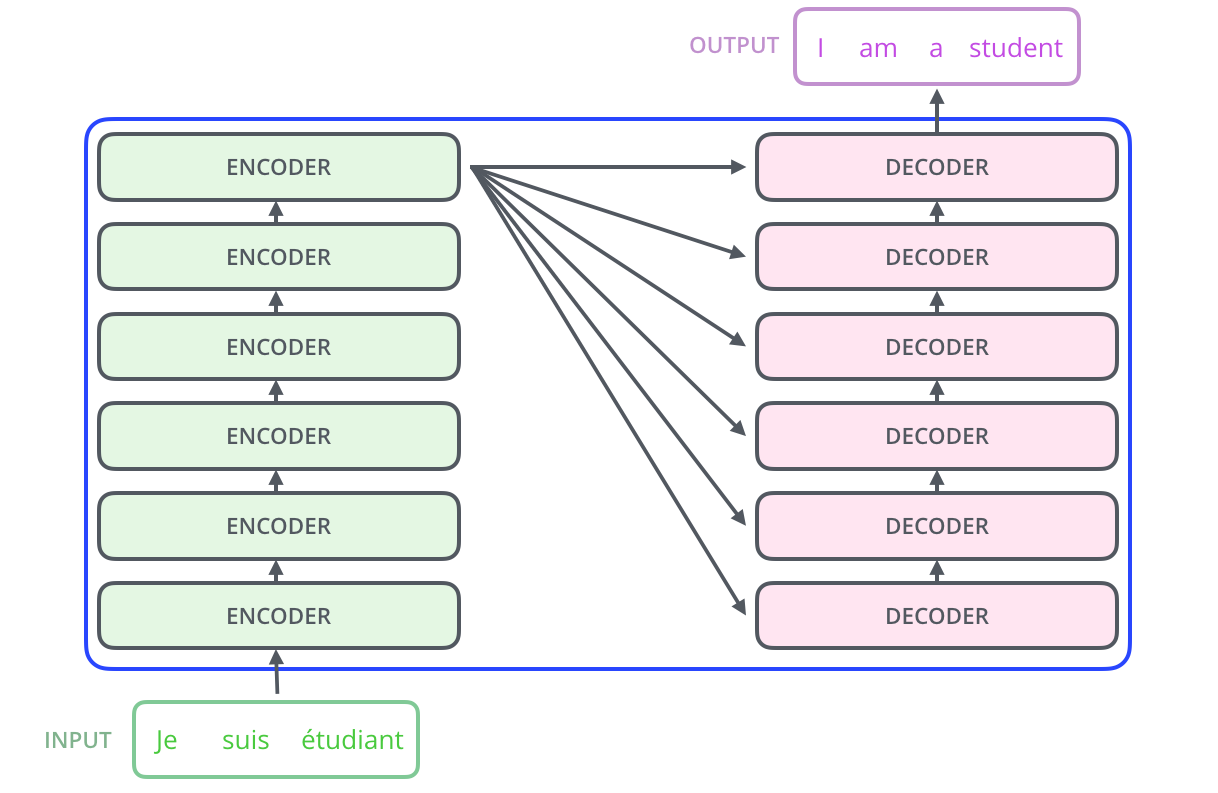
\includegraphics[width=\linewidth]{./assets/images/The_transformer_encoder_decoder_stack.png}
    \caption{Chồng các khối Encoders và Decoders\cite{https://jalammar.github.io/illustrated-transformer/}}
\end{minipage}

\subsubsection{Embedding và Positional Encoding}
\textbf {Input Embedding và Output Embedding}
Trong Transformer, Input Embedding và Output Embedding đều là tầng Embedding
để chuyển đổi đầu vào thành vector với số thực.

Đây là tầng đầu tiên trong kiến trúc Transformer, nhận đầu vào là một
one-hot-encoded vector là một vector có độ dài bằng với số từ trong từ điển,

Mỗi từ đi vào sẽ được tầng này tạo ra một vector đặc, có số chiều nhỏ hơn ban đầu.
\textbf {Positional Encoding}
Kết quả của tầng Input Embedding hoặc Output Embedding
sẽ được đi qua một phép tính Positional Encoding.

\begin{minipage}{\linewidth}
    \captionsetup{type=figure}
    \centering
    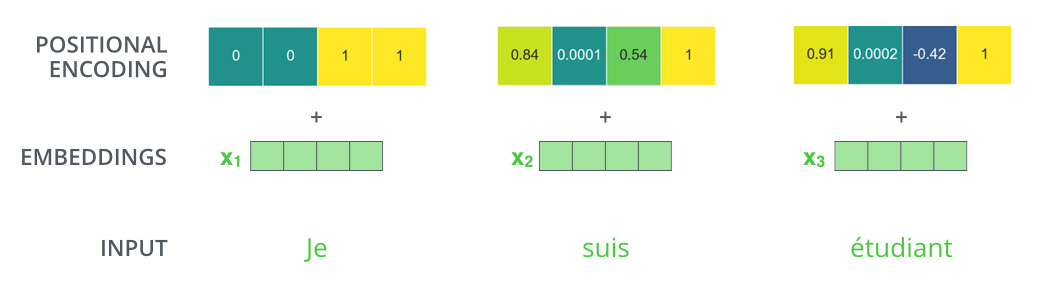
\includegraphics[width=\linewidth]{./assets/images/transformer_input.png}
    \caption{Tầng Input và Output của Transformers\cite{Bramas2021AFV}}
\end{minipage}


Do Transformer không tính toán tuần tự mà xử lý một cách song song , nên nó không có khả năng
nhận biết được vị trí của từ trong câu. Mục tiêu của phép tính
Positional Encoding là để giữ lại vị trí cho câu input, không làm mất thứ tự và ngữ nghĩa câu.

\subsubsection{Khối Multi-Headed Attention}
\textbf{Scaled Dot-Product Attention}
Attention là một cơ chế cho phép mô hình tập trung vào những phần quan trọng của đầu vào (Input) trong quá trình học.
Cơ chế Attention được sử dụng trong nhiều mô hình NLP, bao gồm cả mô hình Transformer.

\begin{minipage}{\linewidth}
    \captionsetup{type=figure}
    \centering
    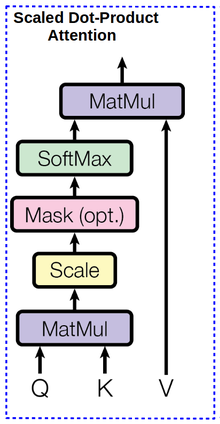
\includegraphics[width=.2\linewidth]{./assets/images/ScaledDotProductAttention.png}
    \caption{Khối ScaleDotProductAttention\cite{DBLP:journals/corr/VaswaniSPUJGKP17}}
\end{minipage}

Đầu vào của Scaled Dot-Product Attention là 3 ma trận Q, K, V có cùng số chiều.

Đầu ra của Scaled Dot-Product Attention là ma trận có cùng số hàng với ma trận Q và cùng số cột với ma trận V thể hiện trọng số attention của nó.

Dữ liệu trong khối này sẽ được xử lý như sau: \begin{itemize}
    \item[--] Hai ma trận Q và K sẽ được nhân lại với nhau, sau đó chia cho căn bậc hai của số chiều
        của ma trận K (tầng Scale) nhằm ngăn giá trị tăng lên quá lớn .
    \item[--] Sau tầng Scale, nếu có tầng Mask thì sẽ được thực hiện để ngăn chặn Attention đến các kết nối không
        hợp lệ (illegal connection).
    \item[--] Sau đó, ma trận sau khi được nhân sẽ được đưa vào hàm softmax để chuẩn hóa giá trị Attention. Giúp mô hình tự tin hơn với các trọng số.
    \item[--] Cuối cùng, ma trận sau khi được chuẩn hóa sẽ được nhân với ma trận V để tạo ra đầu ra của khối Scaled Dot-Product Attention. Đây chính là trọng số Attention của khối.
\end{itemize}

\textbf{Multi-headed Attention}

Thay vì chỉ sử dụng một khối Scaled Dot-Product Attention, Transformer sử dụng
nhiều khối Scaled Dot-Product Attention song song (parallel) để tăng khả năng học của mô hình, hiểu ngữ nghĩa theo nhiều khối.

Đầu ra của mỗi khối Scaled Dot-Product Attention sẽ được nối với nhau và đi qua một tầng Linear để tạo ra đầu ra của khối Multi-Headed Attention.

Kết quả của khối là một ma trận có cùng số hàng với ma trận Q và cùng số cột với ma trận V thể hiện trọng số attention của nó.

\begin{minipage}{\linewidth}
    \captionsetup{type=figure}
    \centering
    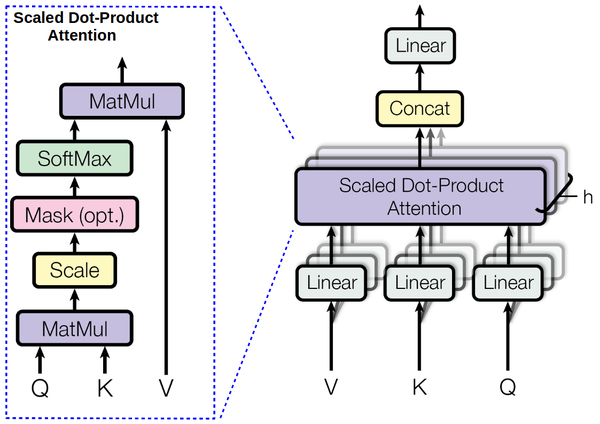
\includegraphics[width=.6\linewidth]{./assets/images/MultiHead.png}
    \caption{Multi-headed Attention\cite{app13148473}}
\end{minipage}

\subsection{Add và LayerNormalization}
Trong Transformer, Add \& Norm được sử dụng để kết hợp thông tin
từ các tầng khác nhau trong mạng. Trong quá trình này, đầu ra của một tầng sẽ được
cộng với đầu vào ban đầu của tầng đó (skip-connection), sau đó chuẩn hóa lại với Layer
Normalization để tạo ra đầu ra cuối cùng.

\begin{minipage}{\linewidth}
    \captionsetup{type=figure}
    \centering
    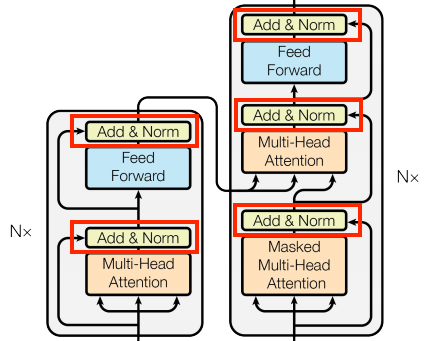
\includegraphics[width=.8\linewidth]{./assets/images/Add+Norm.png}
    \caption{Tầng Add và LayerNormalization\cite{372429372_A_Stock_Price_Prediction_Method_Based_on_BiLSTM_and_Improved_Transformer}}
\end{minipage}
\subsubsection{Add}
Trong bước này, đầu ra của lớp sẽ được cộng với vector
đầu vào ban đầu. Việc cộng này giúp cập nhật thông tin từ các phần khác nhau của kiến
trúc và giúp tránh hiện tượng mất thông tin (Vanishing Gradient) trong quá trình huấn
luyện.

\subsubsection{LayerNormalization}
Sau khi được cộng với đầu vào ban đầu, đầu ra của lớp sẽ được chuẩn hóa lại với
Layer Normalization. Layer Normalization là một phép chuẩn hóa dữ liệu đầu ra của
một tầng theo của ma trận đầu ra. Quá
trình chuẩn hóa giúp cải thiện tính ổn định của mô hình

\subsection{Position-wise Feed Forward Network}
\begin{minipage}{\linewidth}
    \captionsetup{type=figure}
    \centering
    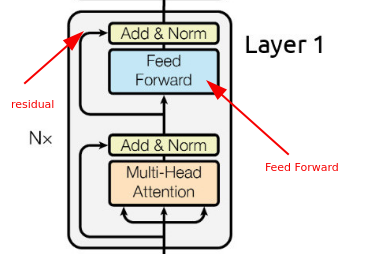
\includegraphics[width=.6\linewidth]{./assets/images/feed-forward-sublayer-in-transformer.png}
    \caption{Khối Position-wise Feed Forward\cite{341553895_Natural_language_processing_system_for_self-reflection_and_peer-evaluation}}
\end{minipage}

Các vector đầu vào (là các vector đại diện cho từ) sẽ được truyền qua tầng Fully Connected Layer với hàm kích hoạt ReLU, và cuối cùng đi qua một tầng Fully ConnectedLayer nữa.
Đầu ra của tầng thứ hai cũng chính ra đầu ra của Position-wise Feed-Forward.

Mục đích chính là xử lý tiếp attention output từ tầng trước đó, giúp mô hình có thể học được các mối quan hệ giữa các từ trong câu.



\subsection{Mô hình SBERT} 
\subsubsection{Độ tương đồng giữa các embedding}

Trong lĩnh vực xử lý ngôn ngữ tự nhiên, một embedding là một biểu diễn vector của một chuỗi, được tạo ra bởi một mô hình học máy. Embedding có thể được tạo ra bằng cách sử dụng các mô hình học máy như Word2Vec, GloVe, FastText, và nhiều mô hình khác.
Ngoài ra, với sự phát triển của các mô hình học sâu và kiến trúc transformer, các embedding có thể được tạo ra bằng cách sử dụng khối encoder các mô hình sử dụng kiến trúc transformer hoặc các mô hình học sâu BERT, GPT, và nhiều mô hình khác.

Để đánh giá độ tương đồng giữa các embedding, chúng ta cần một phương pháp đánh giá độ tương đồng. Một trong những phương pháp đánh giá độ tương đồng giữa các embedding đó là độ tương đồng cosin. Công thức tính độ tương đồng cosin giữa hai embedding $A$ và $B$ được tính như sau:

\begin{equation}
    \text{similarity}(A, B) = \cos(\theta) = \frac{A \cdot B}{\|A\| \|B\|}
\end{equation}

Một số ưu điểm khi sử dụng độ tương đồng cosin để đánh giá độ tương đồng giữa các embedding:
\begin{enumerate}
    \item \textbf{Không Ảnh Hưởng bởi Độ Dài:} Một trong những ưu điểm chính của độ tương đồng cosine là nó không bị ảnh hưởng bởi độ dài của vectơ. Bất kể kích thước của các vectơ, chỉ cần hướng của chúng giống nhau, độ tương đồng cosine sẽ là nhỏ nhất khi chúng đối lập và lớn nhất khi chúng trùng hướng.

    \item \textbf{Đo Lường Hướng Tương Đồng:} Độ tương đồng cosine tập trung vào hướng của vectơ thay vì giá trị tuyệt đối. Điều này làm cho nó thích hợp cho các tác vụ như phân loại văn bản, xác định chủ đề, và tìm kiếm tương đồng ngữ cảnh.

    \item \textbf{Hiệu Quả Cho Dữ Liệu Nhiều Chiều:} Trong không gian chiều cao, nơi mỗi chiều biểu diễn một đặc trưng khác nhau, độ tương đồng cosine thường hiệu quả hơn so với các phương pháp đo tương đồng khác. Điều này giúp giảm hiệu ứng "hiệu ứng chiều cao" khi sử dụng các phương pháp dựa trên khoảng cách Euclidean.
\end{enumerate}

\subsubsection{Siamese Networks}

\begin{minipage}{\linewidth}
    \captionsetup{type=figure}
    \centering
    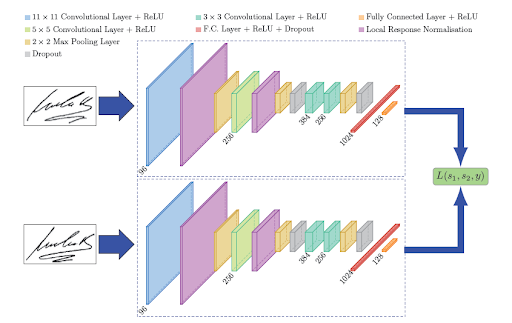
\includegraphics[width=10cm]{./assets/images/1_siamese-network.png}
    \caption{Siamese Networks\cite{https://builtin.com/machine-learning/siamese-network}}
\end{minipage} 

Mạng Siamese là một kiến trúc mạng nơ-ron đặc biệt được thiết kế để xác định mức độ tương đồng giữa hai đối tượng hoặc hai đầu vào. Đặc điểm chính của mạng Siamese là sử dụng hai nhánh đồng nhất (tương tự nhau) chia sẻ trọng số, mỗi nhánh xử lý một đầu vào khác nhau. Mục tiêu của mạng Siamese là học cách biểu diễn và so sánh đặc trưng giữa các cặp đối tượng.

Mạng Siamese thường được sử dụng trong các nhiệm vụ như nhận dạng khuôn mặt, phân loại văn bản, hay tìm kiếm hình ảnh, văn bản tương đồng. Để đạt được mục tiêu này, mạng Siamese thực hiện các bước cơ bản như sau:

\begin{itemize}
    \item[--] \textbf{Trích Xuất Đặc Trưng:} Mỗi nhánh của mạng Siamese nhận một đầu vào và trích xuất đặc trưng từ đối tượng đó bằng cách sử dụng các lớp tích chập và lớp pooling.

    \item[--] \textbf{So Sánh Đặc Trưng:} Các đặc trưng được trích xuất từ cả hai nhánh sau đó được so sánh để đo lường mức độ tương đồng giữa chúng. Thông thường, một hàm khoảng cách như Euclidean hoặc độ tương đồng cosine được sử dụng để đo lường khoảng cách giữa hai vectơ đặc trưng.

    \item[--] \textbf{Huấn Luyện và Tối Ưu Hóa:} Mạng Siamese được huấn luyện bằng cách sử dụng các cặp dữ liệu huấn luyện được gán nhãn với thông tin về mức độ tương đồng. Mục tiêu là tối ưu hóa mô hình để đặc trưng của các cặp giống nhau gần nhau và của các cặp khác nhau xa nhau.
\end{itemize}

Mạng SNN tập trung vào việc cải thiện embedding sao cho các lớp giống nhau sẽ nằm gần nhau hơn. Với việc phải bình phương số lượng dữ liệu để tạo ra các cặp so sánh, việc huấn luyện nó sẽ mất thời gian hơn là phân lớp thông thường.
Chi tiết cách huấn luyện mạng SNN như sau:

\begin{enumerate}
    \item \textbf{Xây dựng} kiến trúc mạng, hàm loss và optimizer.
    \item \textbf{Đưa dữ liệu} 1 trong cặp qua network.
    \item \textbf{Đưa dữ liệu} 2 trong cặp qua network.
    \item \textbf{Tình lỗi} dựa vào output từ dữ liệu 1 và dữ liệu 2
    \item \textbf{Lan truyền ngược} để tính lại đạo hàm của các trọng số.
    \item \textbf{Cập nhật trọng số} bằng optimizer.
\end{enumerate}

\subsubsection{Tổng quan mô hình}
SBERT , hay Sentence-BERT, là một tiến bộ quan trọng trong lĩnh vực xử lý ngôn ngữ tự nhiên (NLP) và biểu diễn văn bản. Được phát triển dựa trên ý tưởng của BERT (Bidirectional Encoder Representations from Transformers), SBERT tập trung vào việc tối ưu hóa biểu diễn cho các câu trong văn bản.

Với nhược điểm về thời gian so sánh giữa các cặp câu của BERT
,phương pháp phổ biến để giải quyết các vấn đề nhóm và tìm kiếm ý nghĩa là ánh xạ mỗi câu vào không gian vectơ sao cho các câu có ý nghĩa tương tự sẽ gần nhau. Các nhà nghiên cứu đã bắt đầu đưa từng câu vào BERT và rút trích các vectơ nhúng cố định cho câu đó. Phương pháp phổ biến nhất là lấy trung bình của lớp đầu ra của BERT (được biết đến là nhúng BERT) hoặc bằng cách sử dụng đầu ra của ký tự đầu tiên (ký tự [CLS]). Nhưng thực nghiệm cho rằng, phương pháp này tạo ra các vectơ nhúng câu khá kém, thường xấp xỉ hoặc kém hơn so với việc lấy trung bình vectơ nhúng GloVe.

Sentence-BERT (SBERT), một phiên bản chỉnh sửa của mạng BERT sử dụng mô hình siamese và triplet với khả năng tạo ra nhúng câu mang ý nghĩa ngữ nghĩa. Điều này cho phép BERT được sử dụng cho một số nhiệm vụ mới, mà cho đến nay chưa áp dụng được cho BERT. Các nhiệm vụ này bao gồm so sánh ý nghĩa ngữ cảnh quy mô lớn, phân nhóm, và truy xuất thông tin thông qua tìm kiếm ý nghĩa ngữ.

\begin{minipage}{\linewidth}
    \captionsetup{type=figure}
    \centering
    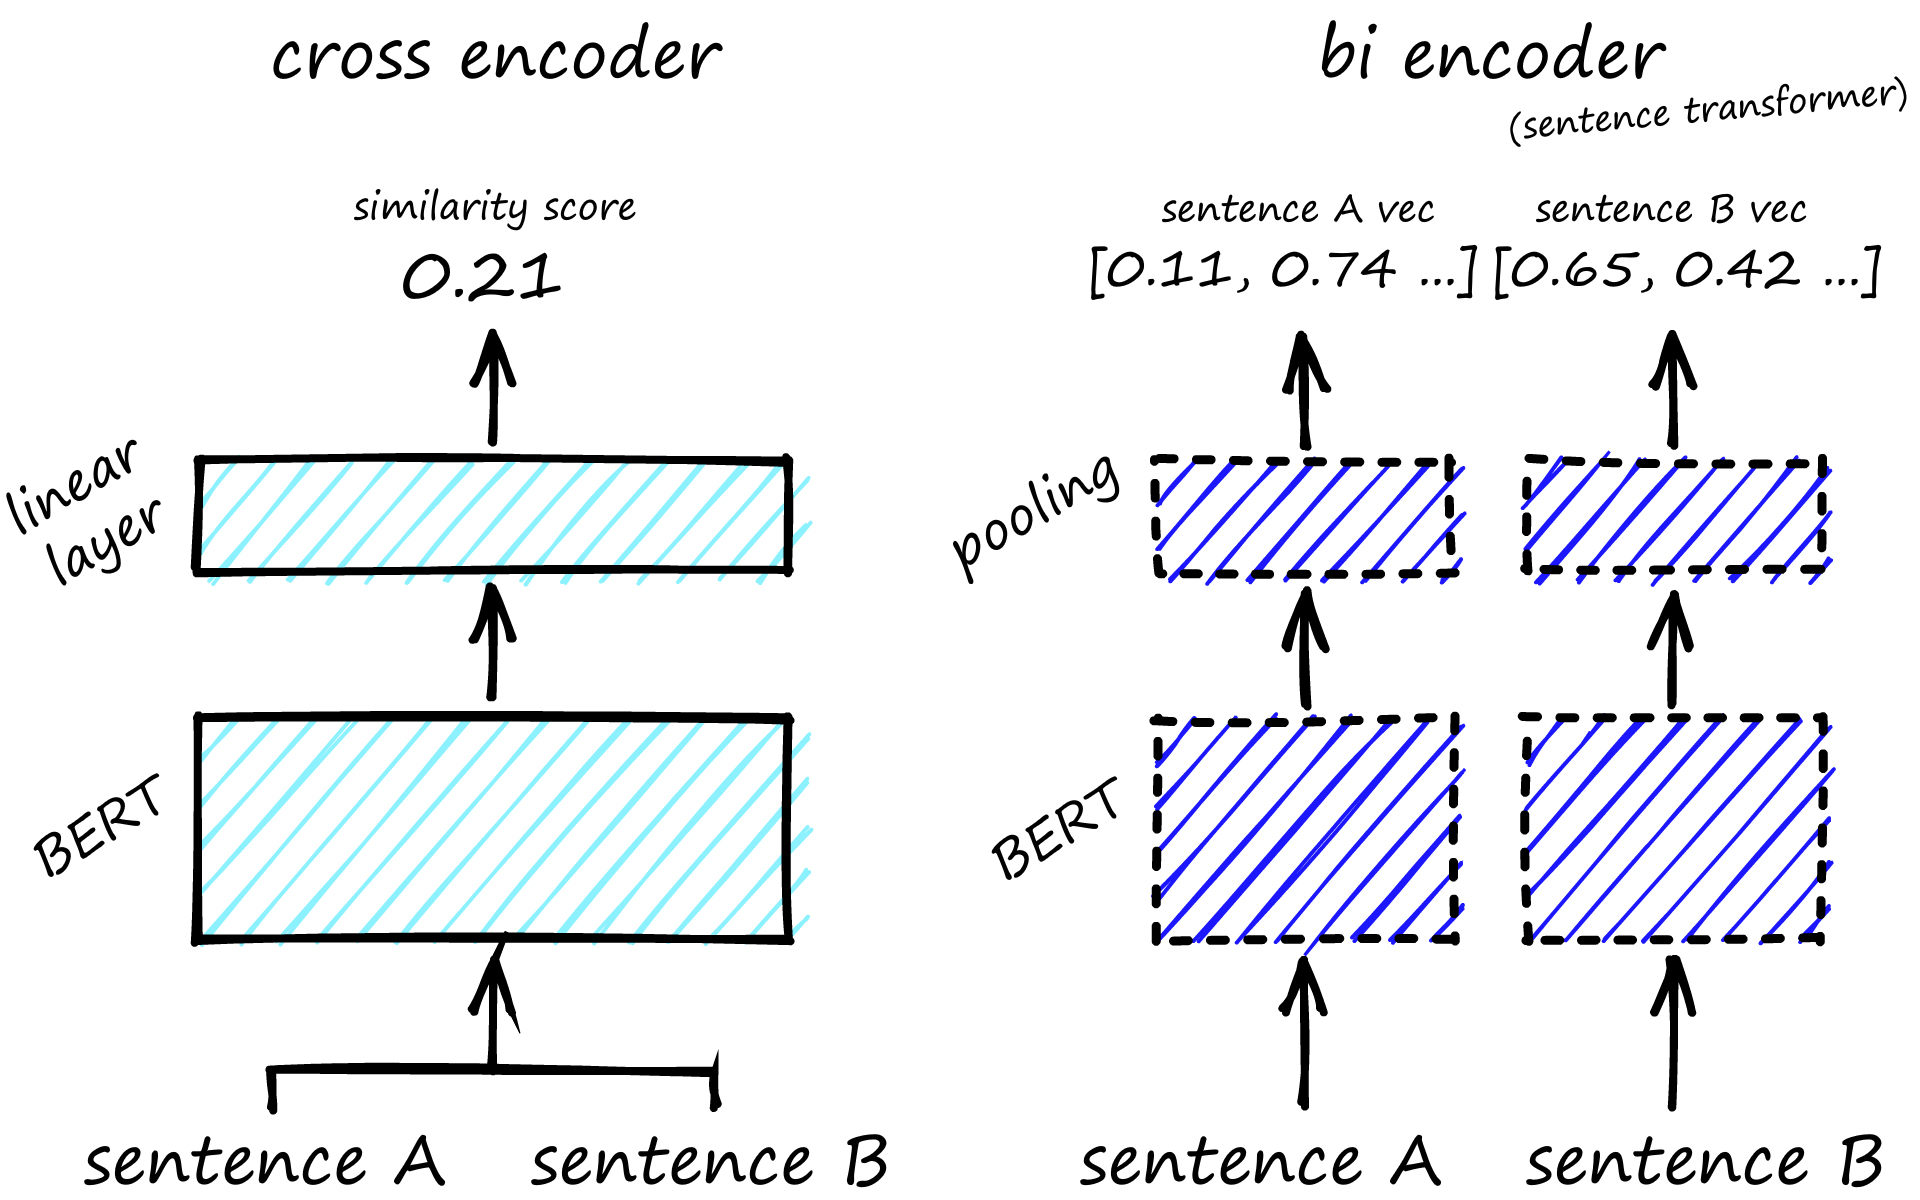
\includegraphics[width=12cm]{./assets/images/sbert1.jpg}
    \captionof{figure}{Sự khác biệt giữa cách tiếp cận của mô hình BERT và SBERT trong bài toán so sánh sự tương đồng ngữ nghĩa}
\end{minipage}

SBERT thêm vào một tầng pooling cho tầng output của BERT để lấy ra được
một embedding vector size cố định cho câu đó. Đã thử nghiệm trên cả 3 cách pooling và chọn phương thức MEAN Pooling:

\begin{itemize}
    \item[--] Sử dụng output của CLS token.
    \item[--] Sử dụng MEAN pooling.
    \item[--] Sử dụng MAX pooling.
\end{itemize}

\subsubsection{Finetune từ BERT, RoBERTa}

Và để fine-tune lại các mô hình BERT và RoBERTa, SBERT sử dụng kiến trúc siamese và triplet network.
Trong quá trình fine-tuning sẽ cập nhật trọng số sao cho các vector embedding đầu ra có ngữ nghĩa và có thể được so sánh bằng cosine similarity.

\begin{multicols}{2}
    \begin{minipage}
        {14cm}
        \captionsetup{type=figure}
        \centering
        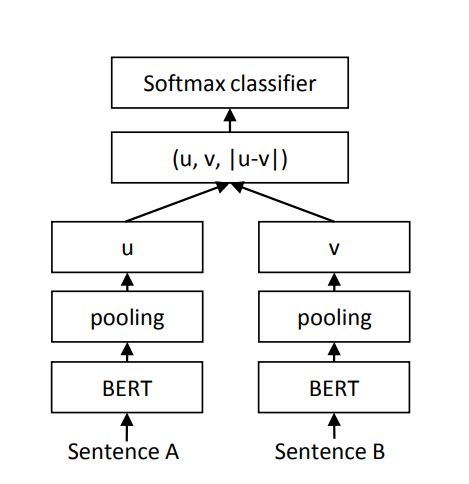
\includegraphics[width=5cm]{./assets/images/sbert-softmax.png}
        \captionof{figure}{SBERT fine-tuned lại BERT sử dụng hàm đánh giá là Softmax Classifier (1)}
        \label{fig:demo-register-1}
    \end{minipage}

    \begin{minipage}
        {14cm}
        \captionsetup{type=figure}
        \centering
        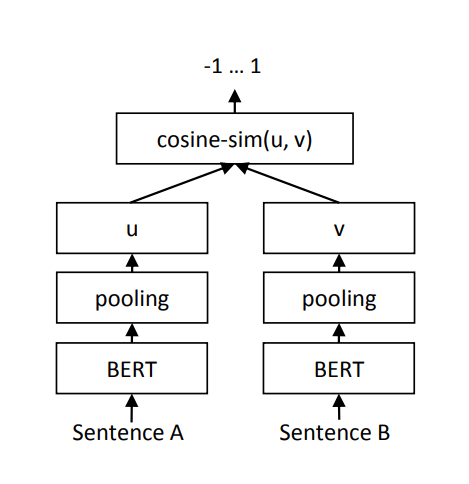
\includegraphics[width=5cm]{./assets/images/sbert-cosine.png}
        \captionof{figure}{SBERT fine-tuned lại BERT sử dụng hàm đánh giá là Cosine Similarity (2)}
        \label{fig:demo-register-2}
    \end{minipage}
\end{multicols}

Trong quá trình fine-tuning, SBERT đã thử nghiệm với 2 hàm đánh giá khác nhau là Softmax Classifier và Cosine Similarity:

\begin{itemize}
    \item[--] Classification: \begin{itemize}
            \item[+] Nối embedding của u, v và phép tính element-wise |u - v|.
            \item[+] Nhân với trọng số  \(W_t \in \mathbb{R}^{3n \times k}\), và cho kết quả đi qua hàm softmax:
                \begin{equation}
                    o = \text{softmax}(W_t(u, v, |u - v|))
                \end{equation}
        \end{itemize}
    \item[--] Regression: Sử dụng cosine similarity để tính độ tương đồng giữa u và v, Sau đó dùng hàm loss là MSE (Mean Square Error) để tính độ lỗi.
\end{itemize}

Huấn luyện SBERT được diễn ra trên sự kết hợp của các tập dữ liệu SNLI \cite{snli:emnlp2015} (Bowman et al., 2015) và Multi-Genre NLI \cite{N18-1101} (Williams et al., 2018).
SNLI là một bộ sưu tập gồm \textbf{570,000} cặp câu được chú thích với các nhãn "contradiction" (mâu thuẫn), "entailment" (hỗ trợ), và "neutral" (trung lập).
MultiNLI chứa \textbf{430,000} cặp câu và bao gồm nhiều thể loại văn bản nói và viết khác nhau. Tinh chỉnh SBERT với một hàm mục tiêu là \textbf{Classification Softmax 3 chiều} trong một epoch. Sử dụng \textbf{batch size là 16}, tối ưu hóa Adam với tốc độ học \textbf{2e-5},
và tăng tốc tốc độ học tuyến tính trên 10\% dữ liệu huấn luyện. Chiến lược pooling sử dụng là \textbf{"MEAN"} (trung bình).

% # TODO: Mô hình BERT

\subsection{Phương pháp RAG}
Phương pháp \ac{rag} là một phương pháp kết hợp giữa phương pháp truy vấn kết hợp và phương pháp sinh câu trả lời.
% # TODO: Phương pháp RAG

\subsection{Xếp hạng lại trong RAG (Re-ranking)}
% # Xếp hạng lại trong RAG (Re-ranking)

\subsection{Truy vấn kết hợp trong RAG (RAG Fusion)}
% # TODO: Truy vấn kết hợp trong RAG (RAG Fusion)

\section{Phương pháp thực hiện}
Trong chương này, đầu tiên, luận văn sẽ trình bày chi tiết phương pháp ứng dụng RAG vào trong hệ thống tư vấn thủ tục hành chính. Hệ thống sử dụng
mô hình SBERT để nhúng văn bản và mô hình ngôn ngữ lớn GPT-3.5 để sinh câu trả lời. Với đầu vào là một câu hỏi của người dùng, 
hệ thống cần trả về một câu trả lời giải quyết được vấn đề của người dùng đi kèm với các trích dẫn thông tin về thủ tục hành chính phù hợp tại Cần Thơ.

Tiếp theo, ở chương này sẽ trình bày từng bước phương pháp xây dựng hệ thống theo kiến trúc Microservices.
Hệ thống cần đảm bảo khả năng mở rộng, cô lập các tính năng và khả năng chịu lỗi cao.

Các bước thực hiện cho hệ thống sẽ được trình bày dựa vào 2 sơ đồ sau:
\subsection{Thu thập dữ liệu}
\subsubsection{Mô tả dữ liệu}
Dữ liệu được sử dụng cho phương pháp RAG - cũng là dữ liệu hệ thống dựa vào để có thể sinh câu trả lời cho câu hỏi họăc tình huống
của người dùng chính là các thủ tục hành chính tại Cần Thơ.

Tất cả các trường dữ liệu thông tin của một thủ tục hành chính đều ở dạng chuỗi. Một thủ tục hành chính bao gồm các thông tin như tên, lĩnh vực, trình tự thực hiện,
cách thức thực hiện, thành phần hồ sơ, căn cứ pháp lý, ... Dữ liệu của một thủ tục hành chính có thể được tìm thấy ở phần phụ lục.

\vspace{0.5cm}
\begin{minipage}{14cm}
    \begin{center}
        \begin{tabular}{ | m{3cm} | m{11cm}| } 
        \cline{1-2} 
        \hline
        \textbf{Trường} & \textbf{Thông tin}\\
        \hline Mã thủ tục & 1.004269.000.00.00.H13 \\
        \hline Tên & Thủ tục cung cấp dữ liệu đất đai (cấp tỉnh) \\
        \hline Trình tự thực hiện & 
                Bước 1:
                - Tổ chức, cá nhân có nhu cầu khai thác dữ liệu đất đai nộp phiếu yêu cầu hoặc gửi văn bản yêu cầu đến Trung tâm Dữ liệu và Thông tin đất đai thuộc Tổng cục Quản lý đất đai hoặc Văn phòng đăng ký đất đai. Đối với địa phương chưa xây dựng cơ sở dữ liệu đất đai, Văn phòng đăng ký đất đai, Ủy ban nhân dân cấp xã;

                Bước 2:
                - Khi nhận được phiếu yêu cầu, văn bản yêu cầu hợp lệ của tổ chức, cá nhân, cơ quan cung cấp dữ liệu đất đai thực hiện việc cung cấp dữ liệu cho tổ chức, cá nhân có yêu cầu khai thác dữ liệu. Cơ quan cung cấp dữ liệu đất đai tiếp nhận, xử lý và thông báo nghĩa vụ tài chính (trường hợp phải thực hiện nghĩa vụ tài chính) cho tổ chức, cá nhân. Trường hợp từ chối cung cấp dữ liệu thì phải có văn bản trả lời nêu rõ lý do;
                
                \begin{center}
                    ...
                \end{center}
                \\
        \hline
        \end{tabular}
    \end{center}
    \captionsetup{type=table}
    \caption{Giới thiệu một thủ tục hành chính}
\end{minipage}

Nguồn dữ liệu sẽ được cào trực tiếp từ hệ thống thông tin giải quyết thủ tục hành chính thành phố Cần Thơ.
Với tổng cộng 1,827 thủ tục hành chính chia vào 99 nhóm dịch vụ công.
\subsubsection{Cào dữ liệu các thủ tục hành chính}
Dữ liệu các thủ tục hành chính sẽ được cào sử dụng thư viện Selenium với ngôn ngữ lập trình Python. Selenium là một thư viện hỗ trợ tự động hóa việc điều khiển trình duyệt web, 
bằng cách mở và điều khiển trình duyệt web bằng Selenium Webdriver.
Quá trình cào dữ liệu sẽ được thực hiện đa luồng, mỗi luồng sẽ điều khiển một trình duyệt web riêng biệt giúp tăng tốc độ cào dữ liệu.

Phương pháp cào dữ liệu sẽ được trình bày dựa vào sơ đồ bên dưới:

\begin{minipage}{\linewidth}
    \centering
    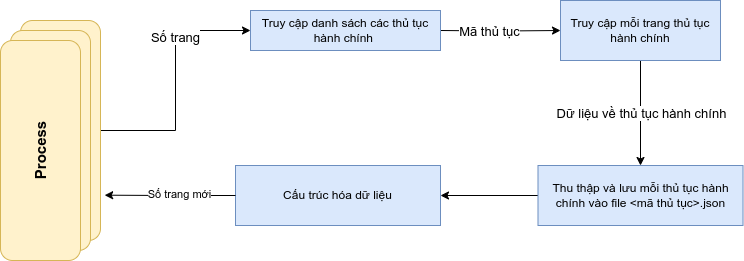
\includegraphics[width=14cm]{./assets/images/procedure-crawl.png}
    \captionsetup{type=figure}
    \caption{Sơ đồ quy trình cào dữ liệu các thủ tục hành chính.}
\end{minipage}

Đầu tiên, webdriver truy cập vào trang dịch vụ công của thành phố Cần Thơ. Tại đây, webdriver sẽ lấy danh sách các nhóm dịch vụ công ở mỗi trang.
Tiếp theo, chương trình chia làm 10 luồng để truy cập vào từng trang chi tiết của thủ tục hành chính, sử dụng thư viện BeautifulSoup để lấy dữ liệu, cấu trúc hóa và lưu vào các tệp file json tương ứng với mã thủ tục.

Trong quá trình thu thập dữ liệu, có một số trường hợp bị lỗi do cách thức hiển thị của trang web. Những trường hợp này sẽ được lưu lại trong tệp log để xử lý thủ công. Dữ liệu thu thập cuối cùng sẽ đầy đủ 1,827 thủ tục hành chính từ hệ thống thông tin giải quyết thủ tục hành chính thành phố Cần Thơ.
\subsection{Tiền xử lý dữ liệu}
% # TODO: Tiền xử lý dữ liệu

\subsection{Xây dựng hệ thống ứng dụng phương pháp RAG}
% # TODO: Xây dựng hệ thống ứng dụng phương pháp RAG

\subsection{Đánh giá kết quả}
% # TODO: Đánh giá kết quả

\subsection{Triển khai hỗ trợ tư vấn thủ tục hành chính}
% # TODO: Triển khai hỗ trợ tư vấn thủ tục hành chính

\section{Kết quả thực nghiệm}
% # TODO: Kết quả thực nghiệm

\chapter{Kết luận}
\section{Kết quả đạt được}
% # TODO: Kết quả đạt được

\section{Hạn chế và hướng phát triển}
% # TODO: Hạn chế và hướng phát triển

\printbibliography

\chapter*{Phụ lục}
\addcontentsline{toc}{chapter}{Phụ lục}

\textbf{File json chứa thông tin một thủ tục hành chính}




\end{document}